\documentclass[10pt]{article}

\usepackage{pgf}
\usepackage{tikz}
\usetikzlibrary{arrows,automata,positioning}
\usepackage[latin1]{inputenc}


\begin{document}

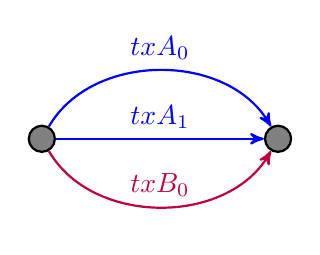
\begin{tikzpicture}[->,>=stealth',auto,node distance=3cm,
  thick,main node/.style={circle,draw,font=\sffamily\Large\bfseries}]

  \node[main node,fill=gray] (1) [] {};
  \node[main node,fill=gray] (2) [right of=1] {};

  \path[every node/.style={font=\sffamily}]
    (1) edge [blue,bend left=60] node [above] {$txA_0$} (2)
    (1) edge [blue] node [above] {$txA_1$} (2)
    (1) edge [purple,bend right=60] node [above] {$txB_0$} (2);
\end{tikzpicture}

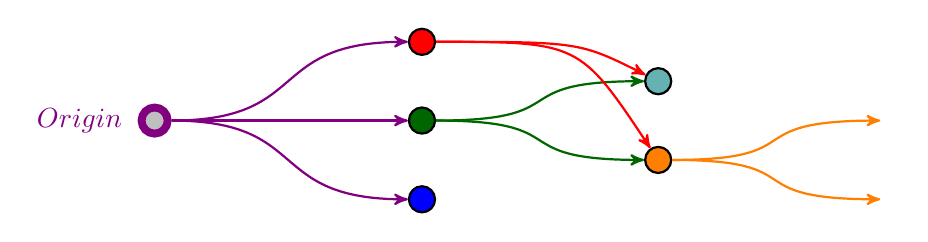
\begin{tikzpicture}[->,>=stealth',auto,node distance=3cm,
  thick,main node/.style={circle,draw,font=\sffamily\Large\bfseries}]
  
  \node[main node,violet,line width=1mm,fill=lightgray,anchor=east] at (0,0) (o) {};
  \node[anchor=east,violet] at (-0.5,0) (x) {$Origin$};
  \node[main node,fill=red,anchor=west] at (3,1) (a) {};
  \node[main node,fill=black!60!green,anchor=west] at (3,0) (b) {};
  \node[main node,fill=blue,anchor=west] at (3,-1) (c) {};
  \node[main node,fill=teal!60,anchor=west] at (6,0.5) (d) {};
  \node[main node,fill=orange,anchor=west] at (6,-0.5) (e) {};
  \node[anchor=west] at (9,0) (f) {};
  \node[anchor=west] at (9,-1) (g) {};
  \draw[->,violet] (o) .. controls ([xshift=2cm] o) and ([xshift=-2cm] a) .. (a);
  \draw[->,violet] (o) .. controls ([xshift=2cm] o) and ([xshift=-2cm] b) .. (b);
  \draw[->,violet] (o) .. controls ([xshift=2cm] o) and ([xshift=-2cm] c) .. (c);
  \draw[->,black!60!green] (b) .. controls ([xshift=2cm] b) and ([xshift=-2cm] d) .. (d);
  \draw[->,black!60!green] (b) .. controls ([xshift=2cm] b) and ([xshift=-2cm] e) .. (e);
  \draw[->,red] (a) .. controls ([xshift=2cm] a)  .. (d);
  \draw[->,red] (a) .. controls ([xshift=2cm] a)  .. (e);
  \draw[->,orange] (e) .. controls ([xshift=2cm] e) and ([xshift=-2cm] f) .. (f);
  \draw[->,orange] (e) .. controls ([xshift=2cm] e) and ([xshift=-2cm] g) .. (g);
\end{tikzpicture}

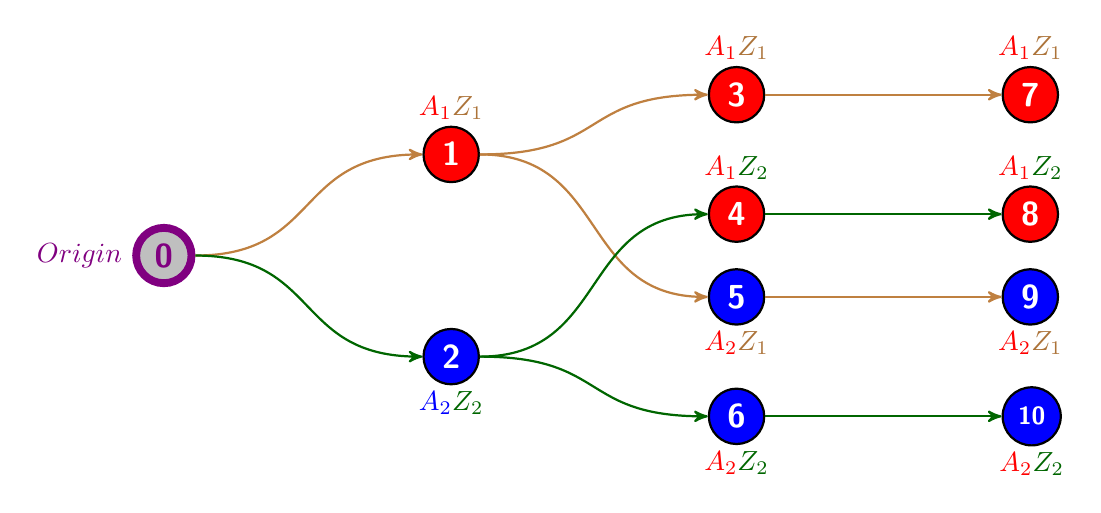
\begin{tikzpicture}[->,>=stealth',auto,node distance=5mm,
  thick,main node/.style={circle,draw,font=\sffamily\large\bfseries}]
  
  \node[main node,violet,line width=1mm,fill=lightgray,anchor=east] (o) {0};
    \node[left=0mm of o,anchor=east,violet] (x) {$Origin$};
  \node[main node,above right=1cm and 3cm of o,fill=red,anchor=west] (S1) {\color{white}1};
  \node[main node,below right=1cm and 3cm of o,fill=blue,anchor=west] (S2) {\color{white}2};
  \node[main node,above right=5mm and 3cm of S1,fill=red,anchor=west] (S3) {\color{white}3};
  \node[main node,below right=5mm and 3cm of S1,fill=red,anchor=west] (S4) {\color{white}4};
  \node[main node,above right=5mm and 3cm of S2,fill=blue,anchor=west] (S5) {\color{white}5};
  \node[main node,below right=5mm and 3cm of S2,fill=blue,anchor=west] (S6) {\color{white}6};
  \node[main node,right=3cm of S3,fill=red,anchor=west] (S7) {\color{white}7};
  \node[main node,right=3cm of S4,fill=red,anchor=west] (S8) {\color{white}8};
  \node[main node,right=3cm of S5,fill=blue,anchor=west] (S9) {\color{white}9};
  \node[main node,right=3cm of S6,fill=blue,anchor=west] (S10) {\color{white}\small 10};
  \node[above=of S1,anchor=north] {\color{red}$A_1\color{black!10!brown}Z_1$};
  \node[below=of S2,anchor=south] {\color{blue}$A_2\color{black!60!green}Z_2$};
  \node[above=of S3,anchor=north] {\color{red}$A_1\color{black!10!brown}Z_1$};
  \node[above=of S4,anchor=north] {\color{red}$A_1\color{black!60!green}Z_2$};
  \node[above=of S7,anchor=north] {\color{red}$A_1\color{black!10!brown}Z_1$};
  \node[above=of S8,anchor=north] {\color{red}$A_1\color{black!60!green}Z_2$};
  \node[below=of S5,anchor=south] {\color{red}$A_2\color{black!10!brown}Z_1$};
  \node[below=of S6,anchor=south] {\color{red}$A_2\color{black!60!green}Z_2$};
  \node[below=of S9,anchor=south] {\color{red}$A_2\color{black!10!brown}Z_1$};
  \node[below=of S10,anchor=south] {\color{red}$A_2\color{black!60!green}Z_2$};
  \draw[->,brown] (o) .. controls ([xshift=2cm] o) and ([xshift=-2cm] S1) .. (S1);
  \draw[->,brown] (S1) .. controls ([xshift=2cm] S1) and ([xshift=-2cm] S3) .. (S3);
  \draw[->,brown] (S1) .. controls ([xshift=2cm] S1) and ([xshift=-2cm] S5) .. (S5);
  \draw[->,black!60!green] (S2) .. controls ([xshift=2cm] S2) and ([xshift=-2cm] S4) .. (S4);
  \draw[->,black!60!green] (S2) .. controls ([xshift=2cm] S2) and ([xshift=-2cm] S6) .. (S6);
  \draw[->,black!60!green] (o) .. controls ([xshift=2cm] o) and ([xshift=-2cm] S2) .. (S2);
  \draw[->,brown] (S3) to (S7);
  \draw[->,brown] (S5) to (S9);
  \draw[->,black!60!green] (S4) to (S8);
  \draw[->,black!60!green] (S6) to (S10);
\end{tikzpicture}

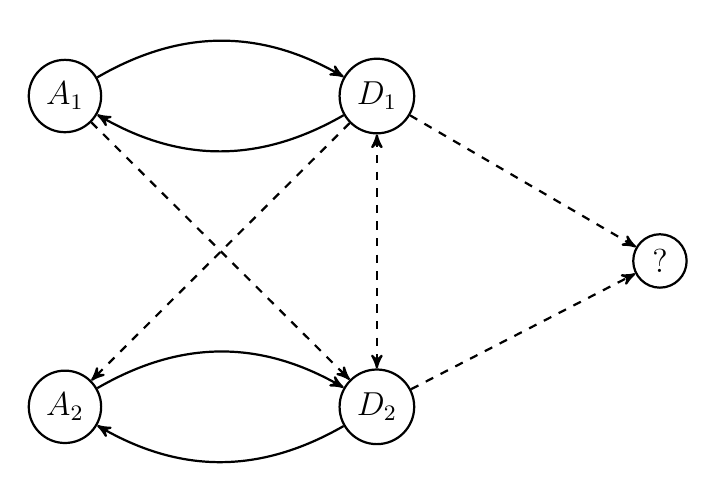
\begin{tikzpicture}[->,>=stealth',auto,node distance=30mm,
  thick,main node/.style={circle,draw,font=\sffamily\large\bfseries}]
    \node[main node](A1){$A_1$};
    \node[main node,below=of A1](A2){$A_2$};
    \node[main node,right=of A1](D1){$D_1$};
    \node[main node,right=of A2](D2){$D_2$};
    \node[main node,below right=15mm and 30mm of D1](X){\large $?$};
    \path (A1) [bend left] edge (D1)
          (D1) [bend left] edge (A1)
          (A2) [bend left] edge (D2)
          (D2) [bend left] edge (A2)
    ;
    \path[<->]
          (D1) [dashed] edge (D2)
    ;
    \path
          (A1) [dashed] edge (D2)
          (D1) [dashed] edge (A2)
          (D1) [dashed] edge (X)
          (D2) [dashed] edge (X)
    ;
           
\end{tikzpicture}

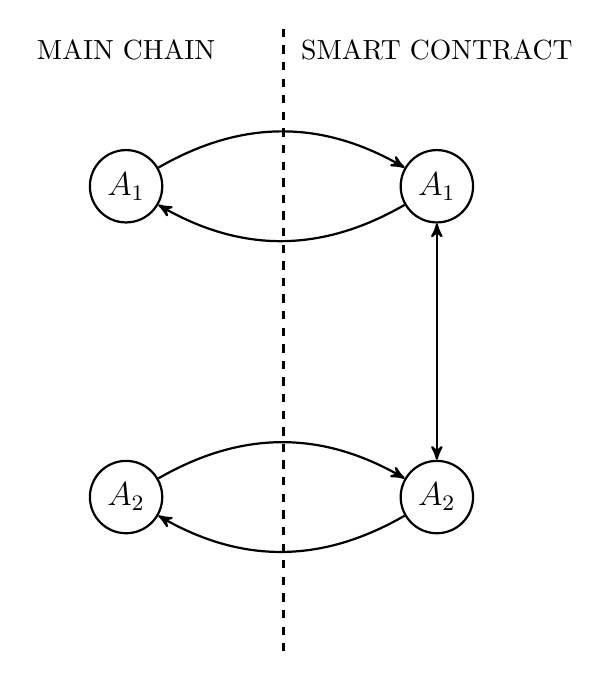
\begin{tikzpicture}[->,>=stealth',auto,node distance=3,
  thick,main node/.style={circle,draw,font=\sffamily\large\bfseries}]
    \node[main node](A1){$A_1$};
    \node[main node,below=of A1](A2){$A_2$};
    \node[main node,right=of A1](D1){$A_1$};
    \node[main node,right=of A2](D2){$A_2$};
    \node[above=1 of A1]{MAIN CHAIN};
    \node[above=1 of D1]{SMART CONTRACT};
    \path (A1) [bend left] edge (D1)
          (D1) [bend left] edge (A1)
          (A2) [bend left] edge (D2)
          (D2) [bend left] edge (A2)
    ;
    \path[<->]
          (D1) edge (D2)
    ;
    \draw[-,dashed] (2,2) -- (2,-6);

\end{tikzpicture}

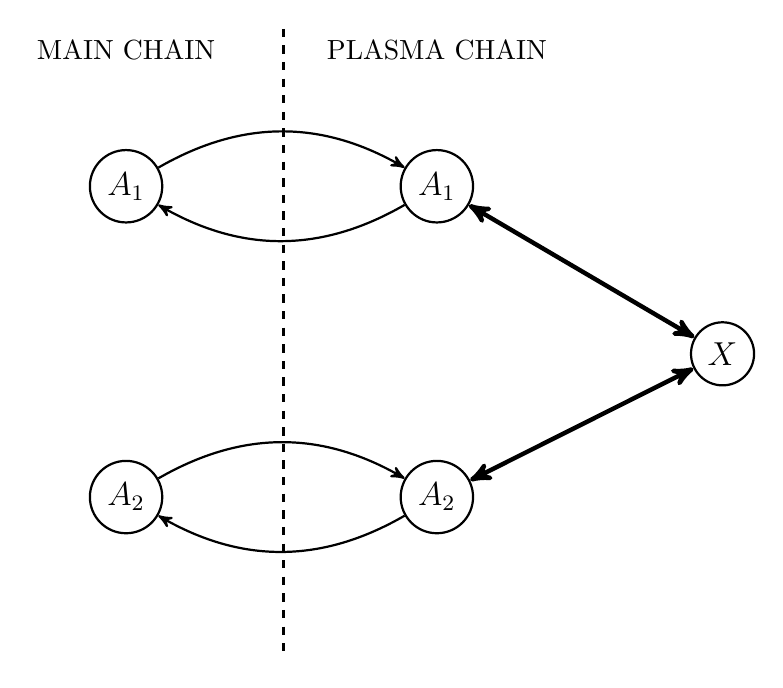
\begin{tikzpicture}[->,>=stealth',auto,node distance=3,
  thick,main node/.style={circle,draw,font=\sffamily\large\bfseries}]
    \node[main node](A1){$A_1$};
    \node[main node,below=of A1](A2){$A_2$};
    \node[main node,right=of A1](D1){$A_1$};
    \node[main node,right=of A2](D2){$A_2$};
    \node[main node,below right=15mm and 30mm of D1](X){$X$};
    \node[above=1 of A1]{MAIN CHAIN};
    \node[above=1 of D1]{PLASMA CHAIN};
    \path (A1) [bend left] edge (D1)
          (D1) [bend left] edge (A1)
          (A2) [bend left] edge (D2)
          (D2) [bend left] edge (A2)
    ;
    \path[<->]
          (D1) [ultra thick] edge (X) 
          (D2) [ultra thick] edge (X)
    ;
    \draw[-,dashed] (2,2) -- (2,-6);

\end{tikzpicture}

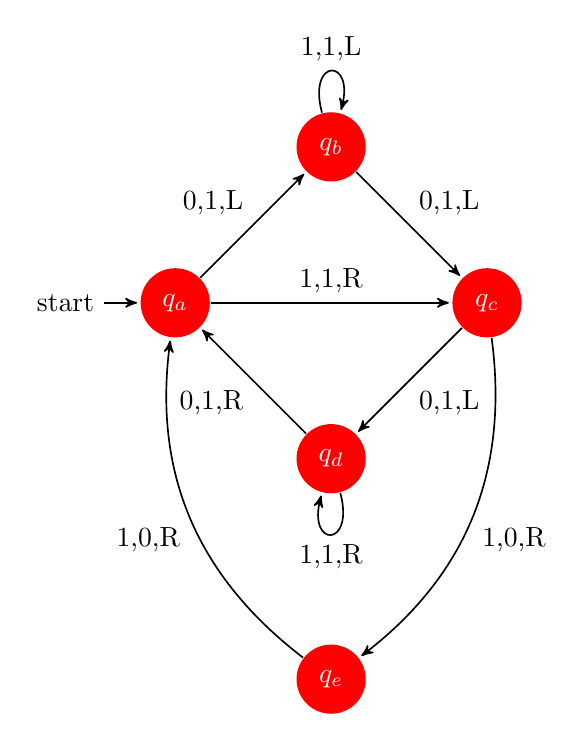
\begin{tikzpicture}[->,>=stealth',shorten >=1pt,auto,node distance=2.8cm,
                    semithick]
  \tikzstyle{every state}=[fill=red,draw=none,text=white]

  \node[initial,state] (A)                    {$q_a$};
  \node[state]         (B) [above right of=A] {$q_b$};
  \node[state]         (D) [below right of=A] {$q_d$};
  \node[state]         (C) [below right of=B] {$q_c$};
  \node[state]         (E) [below of=D]       {$q_e$};

  \path (A) edge              node {0,1,L} (B)
            edge              node {1,1,R} (C)
        (B) edge [loop above] node {1,1,L} (B)
            edge              node {0,1,L} (C)
        (C) edge              node {0,1,L} (D)
            edge [bend left]  node {1,0,R} (E)
        (D) edge [loop below] node {1,1,R} (D)
            edge              node {0,1,R} (A)
        (E) edge [bend left]  node {1,0,R} (A);
\end{tikzpicture}

\end{document}